\documentclass[11pt, a4paper, oneside]{article}
\usepackage{worksheet}
\usepackage{subfiles}
\usepackage{physics}
\usepackage{siunitx}
\usepackage{comment}

\author{ID:}
\date{Final Partial}
\title{Roller Coaster project}
\subject{Name: }
\class{Calculus I}

\begin{document}
    \maketitle
    %\testheader[100]{remarks}

    \section*{Instructions}
    In this project, you will use higher-order derivatives to propose a solution to finish a roller coaster track.
    Follow each one of the following tasks to achieve the goal.
    This project is done individually.
    You can ask for help from your colleagues and the professor.
    For each session, you will have between 10 and 25 minutes to work on this project.
    Write your final answer in the boxes.
    All procedures will be on external sheets of paper.

    \section*{Description of the goals}

    In Figure~\ref{fig:sketch}, the four points where the functions meet are shown. 
    Your task is to find the coefficients of a cubic function that connects the point (10,0) to the point (30,20), and the coefficients of a sine function that connects the point (50,50) to (100,0). 
    The functions must be tangent (i.e., have first-order contact) at the corresponding connection points. 
    This means that at those points, the two functions share the same value and the same first derivative.

    \begin{figure}[ht!]
        \centering
        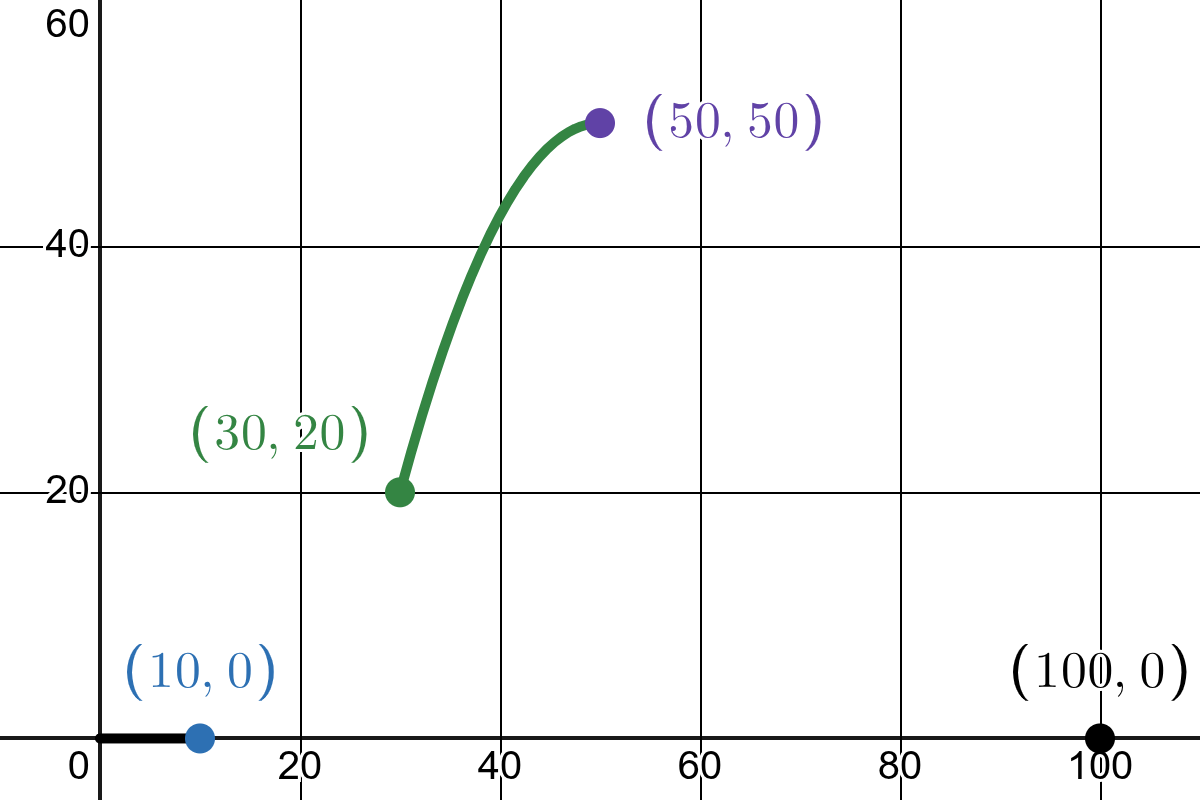
\includegraphics[width=0.85\textwidth]{figures/trayectoria-hueco.png}
        \caption{Sketch of the roller coaster.}\label{fig:sketch}
    \end{figure}

    \newpage

    The final answer is going to be a stepwise function,
    \begin{gather*}
        R(x) = 
        \left\{
            \begin{array}{cc}
                0 & x\in\qty[0,10] \\
                f(x) & x\in\qty[10,30] \\
                g(x) & x\in\qty[30,50] \\
                h(x) & x\in\qty[50,100]
            \end{array}
        \right.
    \end{gather*}

    The function that connect the point \((30,20)\) with the point \((50,50)\) is given by
    \begin{gather*}
        g(x) = -\frac{3}{40}(x-50)^2 + 50.
    \end{gather*}
    The following instructions are going to help you to find the functions $f(x)$ and $h(x)$ that meets the requeriments.

    \subsection*{Find the cubic function}

    This first set of tasks will allow you to find the coefficients of the following cubic function
    \begin{gather*}
        f(x) = a\qty(x-h)^3.
    \end{gather*}

    \singletask[]{Find \(h\).}
    Equate \(f(x)\) to the point \((10,0)\) and solve for \(h\).

    \boxarea[2cm]

    \singletask[]{Compute derivatives. Find $a$ part 1.}
    Compute the derivative of \(f(x)\) and \(g(x)\).
    
    \boxarea[2cm]

    \singletask[]{Restriction of first-order contact. Find $a$ part 2.}
    Equate \(f'(x)\) with \(g'(x)\) at $x=30$ and solve for $a$.
    
    \boxarea[2cm]

    \singletask[]{First answer}
    Write the function \(f(x)\) with the values.    
    
    \boxarea[2cm]

    \singletask[]{Test continuity at \((10,0)\) and \((30,20)\)}
    Evaluate the function \(f(x)\) at the given points and show that is congruent.
    
    \boxarea[2cm]

    \singletask[]{Test first-order constact at \((10,0)\) and \((30,20)\)}
    Evaluate \(f'(x)\) at the given points and show that is congruent.
    
    \boxarea[2cm]

    If you don't get the expected values, go back and check your procedures or start over.

    \subsection*{Find the sine function}

    This second set of tasks will allow you to find the coefficients of the following trigonometric function
    \begin{gather*}
        h(x) = a\sin\qty[\omega x +h] + k.
    \end{gather*}

    \singletask[]{Compute derivatives.}
    Compute the derivative of \(h(x)\)

    \boxarea[2cm]

    \singletask[]{Restriction of first-order contact. Find $w$ part 1.}
    Equate \(h'(x)\) with \(g'(x)\) at \((50,50)\) and solve for $h$

    \boxarea[2cm]

    \singletask[]{Restriction of first-order contact. Find $w$ part 2.}
    Equate \(h'(x)\) to \(0\) at \((100,0)\) and solve for $h$. 
    Add \(\pi\) to the solution.

    \boxarea[2cm]

    \singletask[]{Restriction of first-order contact. Find $w$ part 3.}
    Equate the previous equations and solve for \(\omega\) 

    \boxarea[2cm]

    \singletask[]{Restriction of first-order contact. Find $h$ part 4.}
    Use the value \(\omega\) to find \(h\).

    \boxarea[2cm]

    \singletask[]{Continuity at \(100,0\)}
    Evaluate the function \(h(x)\) at \(100,0\) and solve for \(a\).
    
    \boxarea[2cm]

    \singletask[]{Continuity at \(50,50\)}
    Evaluate the function \(h(x)\) at \(50,50\) and solve for \(a\) and \(k\).
    
    \boxarea[2cm]

    \singletask[]{Second answer}
    Write the function \(h(x)\) with the values.    
    
    \boxarea[2cm]

    \singletask[]{Test continuity at \((50,50)\) and \((100,0)\)}
    Evaluate the function \(h(x)\) at the given points and show that is congruent.
    
    \boxarea[2cm]

    \singletask[]{Test first-order constact at \((50,50)\) and \((100,0)\)}
    Evaluate \(h'(x)\) at the given points and show that is congruent.
    
    \boxarea[2cm]

    If you don't get the expected values, go back and check your procedures or start over.


\end{document}
